\documentclass[../../main.tex]{subfiles}

\begin{document}
    \subsubsection{Einfluss des Messmodus}
        Im Folgenden soll kurz auf die beiden Messmodi \glqq{}switched mode\grqq{} und \glqq{}signal mode\grqq{} eingegangen werden.
        \begin{figure}[H]
            \centering
            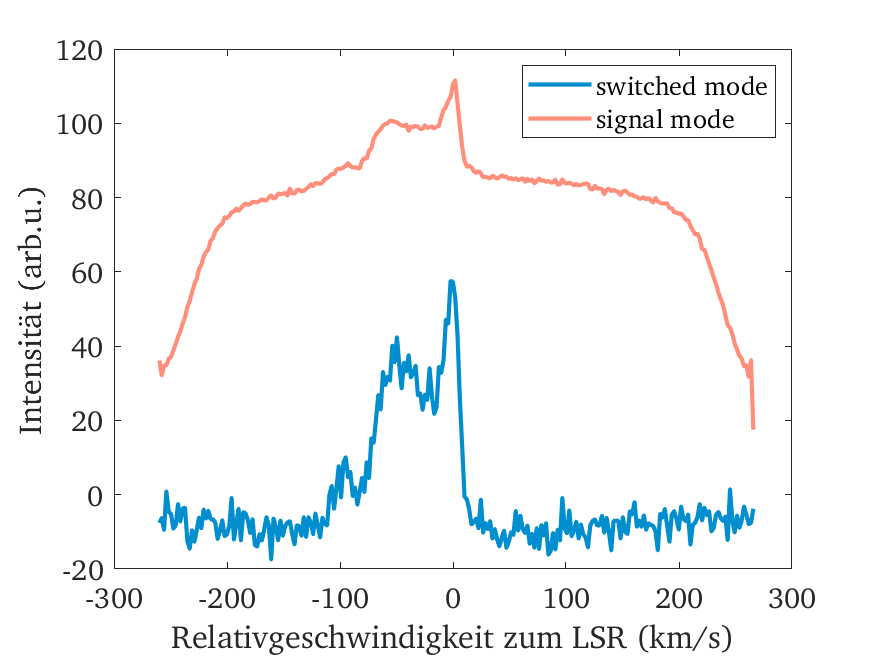
\includegraphics[width=0.75\textwidth]{Bilddateien/Modi/Fig_10.png}
            \caption{Vergleich zwischen den beiden Messmodi. Es ist deutlich zu erkennen, dass das Signal und dessen Peaks, deren Position für die spätere Auswertung relevant ist, im \glqq{}switched mode\grqq{} besser zu erkennen ist.}
            \label{fig:TT:MessModi}
        \end{figure}
        In \autoref{fig:TT:MessModi} werden die Messmodi verglichen. Dabei wird das selbe Objekt angefahren und eine Messung bei $\SI{1420}{\mega \hertz}$ durchgeführt. Es ist zu erkennen, dass im \glqq{}switched mode\grqq{} der Hintergrund vom Messsignal abgezogen wird. Das geschieht in dem bei einer etwas höheren Frequenz ein zweites Spektrum aufgenommen und von der Messung bei $\SI{1420}{\mega \hertz}$ abgezogen wird. Bei dieser Methode wird davon ausgegangen, dass die Hintergrundintensität aus der Charakteristik der Antenne stammt und keine weiteren Quellen hat. Da die Intensität im \glqq{}switched mode\grqq{} ins negative geht, ist zu erkennen, dass diese Annahme nicht vollständig zutrifft. Für die Messung der Relativgeschwindigkeiten der Milchstraße, die im folgenden Abschnitt ausgewertet werden, ist die absolute Intensität allerdings nicht von Interesse. Für diese Messung, ist es wichtig die Positionen der Peaks auf der x-Achse erkennen zu können. Dazu muss lediglich das Verhältnis von Peaksignal zum Hintergrund genügend groß sein, was mit der Methode des \glqq{}switched mode\grqq{} gut funktioniert.

    \subsubsection{Einfluss der Integrationszeit}
    Um in den folgenden Kapiteln zeitlich-qualitativ optimierte Ergebnisse aus den Messungen zu erhalten, untersuchen wir das Verhalten des Teleskops SALSA in Abhängigkeit von der Zeitmittelung. Hierzu betrachteten wir bereits am Experimenttag qualitativ die Rauschausprägungen bei $\delta t\in\{\SI{1}{\s},\SI{3}{\s},\SI{10}{\s},\SI{30}{\s},\SI{100}{\s},\SI{300}{\s}\}$ und vergleichen diese untereinander. Dabei schauen wir mit dem Teleskop in Richtung $l = \SI{100}{\degree}$ und $b = \SI{0}{\degree}$ im \emph{switched mode}.
    \begin{figure}[H]
        \centering
        \includegraphics[width=0.8\textwidth]{Bilddateien/Signalanalyse/spectrum_64931_64936.pdf}
        \caption{Vergleich des best- und worst-case Spektrums bei $\delta t = \SI{1}{\s}$ und $\delta t = \SI{300}{\s}$. Dabei meinen wir mit \enquote{rel. velocity} stets die Relativgeschwindigkeit zum \emph{local standard of rest} (LSR), also das Sonnenruhesystem.}
        \label{fig:bestworstcomp}
    \end{figure}
    In Abbildung \ref{fig:bestworstcomp} vergleichen wir den kürzesten und längsten der getesteten Belichtungswerte. Hierbei fällt die zunehmende Glattheit der Spektren auf, was grundsätzlich der Auswertung zugute kommt, jedoch in Randfällen ebenfalls mögliche dicht beieinanderliegende oder miteinander verschränkte Peaks aufweichen lassen könnte. Da wir in der Auswertung unten ebenfalls mit einem Glättungsalgorithmus arbeiten werden, genügen wir uns der in der Versuchsanleitung \cite{doc:SALSAStudentManual} angegebenen Zeit von $\delta t = \SI{60}{\s}$, welche wir in Abbildung \ref{fig:nexttime100} mit unserem nächstgemessenen Wert vergleichen.
    \begin{figure}[H]
        \centering
        \includegraphics[width=0.8\textwidth]{Bilddateien/Signalanalyse/spectrum_64935.pdf}
        \caption{Nächster Vergleichswert zu unser tatsächlich gewählten Belichtungszeit von $\delta t = \SI{60}{\s}$.}
        \label{fig:nexttime100}
    \end{figure}
    % Aus Interesse schalten wir in einer weiteren Messung den Messmodus des Teleskops von \emph{switched} auf \emph{signal} um und erhalten das in Abbildung \ref{fig:signalmode} dargestellte Spektrum. Hierbei fällt auf, dass die Peaks im Vergleich zu Abbildung \ref{fig:nexttime100} in einem deutlichen Hintergrundsignal verschoben sind und drastisch an Eigenauflösung eingebüßt haben. Den Berg des Hintergrundsignals erklären wir uns durch optisch-geometrische Beugungen und Interferenzen innerhalb der Teleskopschüssel. Insgesamt ist das so erhaltene Signal nicht zur Auswertung geeignet und wir bleiben bei unserem gewählten Messmodus \enquote{\emph{switched}}.

    % \begin{figure}[H]
    %     \centering
    %     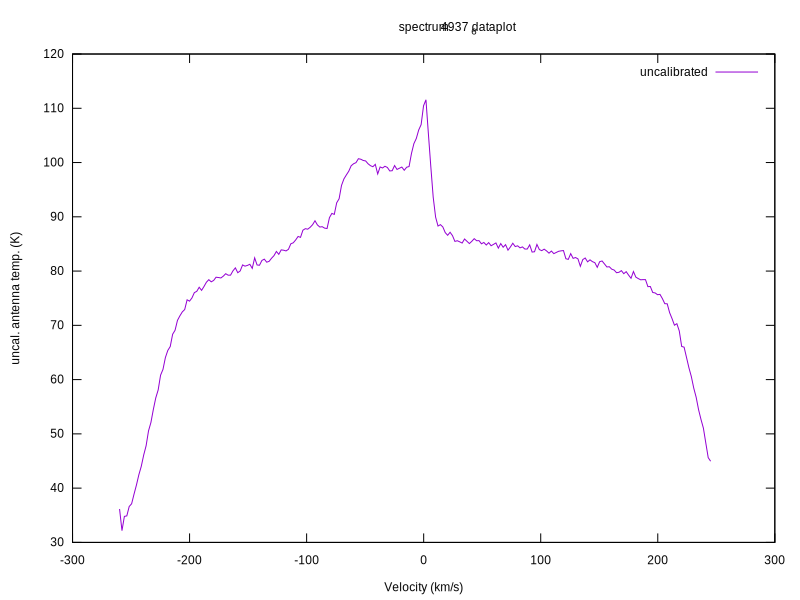
\includegraphics[width=0.8\textwidth]{Bilddateien/Signalanalyse/spectrum_64937.pdf}
    %     \caption{Spektrum bei $\delta t = \SI{100}{\s}$ im \emph{signal mode}.}
    %     \label{fig:signalmode}
    % \end{figure}
    
\end{document}